% 第 20 题椭圆图：按固定源内容流矢量层精确值复刻（1 pt → 0.03515 cm，与全库同制）。
% 原点取 x 轴负端 x=616.4024 pt、y 轴下端 y（顶向下）=289.6055 pt；y 向上。
% 源实测（figure-inventory §4）：椭圆中心 (76.5078, 56.6719)、半轴 a=56.6719 / b=40.0664、
% 线宽 0.7967 bp（其余线的 2 倍，全卷唯一加粗——突出二次曲线，照源）；x 轴左端过原点、
% 右至箭尖 +153.0156（左右对称外伸 76.5078，但左端不画箭头、右端画）；y 轴下外伸 56.6719、
% 上至箭尖 +116.1797；过 P 的割线 (13.4882,37.6914)–(104.2734,108.6563) 长 115.23；
% 全图 4 描边 + 2 纯填充箭头，无虚线、无点标记。
% 源内异常（照源复刻、已登记）：割线与 y 轴交点实测在原点上方 60.7337（非 P 的 56.6719，
% 差 1.94 pt）——图意「过 P 的动直线」，照源实测端点抄录。
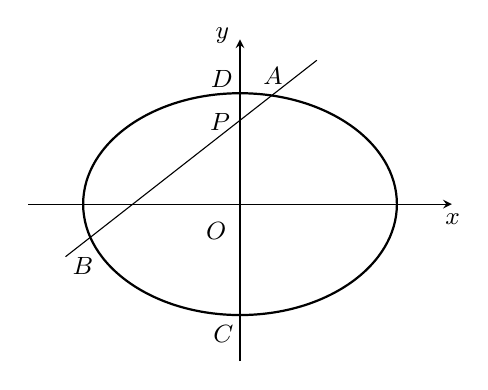
\begin{tikzpicture}[x=0.03515cm,y=0.03515cm,>=stealth,every node/.style={font=\small,inner sep=0pt}]
% ===== 椭圆（4 段贝塞尔，线宽 0.7967 全卷唯一加粗）=====
\draw[line width=0.7967bp] (76.5078,56.6719) ellipse [x radius=56.6719, y radius=40.0664];
% ===== 两轴与箭头 =====
\draw[line width=0.3983bp] (0,56.6719)--(149.4296,56.6719);      % x 轴（右端直线段）
\draw[->,line width=0.3983bp] (149.4296,56.6719)--(153.0156,56.6719); % x 轴箭头（照源独立填充三角，此处并入线端）
\draw[line width=0.3983bp] (76.5078,0)--(76.5078,112.5938);       % y 轴（上端直线段）
\draw[->,line width=0.3983bp] (76.5078,112.5938)--(76.5078,116.1797); % y 轴箭头
% ===== 过 P 的割线 =====
\draw[line width=0.3983bp] (13.4882,37.6914)--(104.2734,108.6563);
% ===== 标签（照源字形盒中心定位）=====
\node at (70.1180,117.6060) {\(y\)};
\node at (88.4580,103.1360) {\(A\)};
\node at (69.9180,101.9860) {\(D\)};
\node at (69.3280,86.1760) {\(P\)};
\node at (153.3080,51.0960) {\(x\)};
\node at (67.9280,47.0060) {\(O\)};
\node at (19.7880,34.4360) {\(B\)};
\node at (70.5480,9.7260) {\(C\)};
\end{tikzpicture}
